\chapter{Przykład sprawozdania}
\label{cha:Lab001}
\makeatletter


% *********************************************************************
% w poniższej metryczce należy uzupełnić informacje o:
% - temacie ćwiczenia
% - numer ćwiczenia
% - numer grupy laboratoryjnej
% - numer zespołu
% - datę wykonania ćwiczenia oraz oddania ćwiczenia.
% *********************************************************************

\begin{table}[H]
    \centering
    \renewcommand{\tabularxcolumn}[1]{m{#1}}  % Dostosowanie kolumny do zawartości
    \newcolumntype{C}{>{\centering\arraybackslash}X}
    \begin{tabularx}{\linewidth}{|C|C|}
        \hline
        \multicolumn{2}{|c|}{\makecell{\textbf{\Large{Biometryczne Systemy Zabezpieczeń}} \\ \textbf{Ćwiczenia Laboratoryjne}}} \\ \hline
        \multicolumn{1}{|l|}{Temat}                    &                           \\ \hline
        \multicolumn{1}{|l|}{Ćwiczenie nr:}                    &      XX                   \\ \hline
        \multicolumn{1}{|l|}{Autorzy:}                         &   \@author                              \\ \hline
        \multicolumn{1}{|l|}{Grupa laboratoryjna}                       &       XX               \\ \hline
        \multicolumn{1}{|l|}{Zespół nr. }                       &    XX                  \\ \hline
        \multicolumn{1}{|l|}{Data wykonana ćwiczenia}         &  XX.XX.XXXX     \\ \hline
        \multicolumn{1}{|l|}{Data oddania ćwiczenia  }         &   XX.XX.XXXX     \\ \hline
    \end{tabularx}
\end{table}


\section{Cel ćwiczenia}
Celem ćwiczenia jest analiza histogramu obrazu biometrycznego, jego zastosowanie w poprawie jakości obrazu oraz segmentacji. Zostaną wykorzystane operacje przetwarzania histogramu, takie jak wyrównywanie histogramu oraz binaryzacja obrazu na podstawie progowania.

\section{Wstęp teoretyczny}
Histogram obrazu to funkcja przedstawiająca rozkład wartości pikseli w obrazie. Może być wykorzystywany do:
\begin{itemize}
    \item Poprawy kontrastu obrazu (rozciąganie histogramu, wyrównywanie histogramu),
    \item Segmentacji obrazu na podstawie progów jasności (np. metoda Otsu),
    \item Analizy jakości obrazu, w tym identyfikacji prześwietlonych lub niedoświetlonych obszarów.
\end{itemize}

Histogram w obrazie monochromatycznym można obliczyć za pomocą funkcji $h(k)$, określającej liczbę pikseli o poziomie jasności $k$:
\begin{equation}
h(k) = \sum_{(x,y) \in \Omega} \delta(I(x,y) - k),
\end{equation}
gdzie $\delta$ to funkcja Kroneckera, a $\Omega$ oznacza zbiór pikseli w obrazie.

\section{Opis wykorzystywanego oprogramowania i narzędzi}
Do przeprowadzenia eksperymentu wykorzystano środowisko MATLAB oraz bibliotekę Image Processing Toolbox. Kluczowe funkcje wykorzystane w analizie to:
\begin{itemize}
    \item \texttt{imhist} - obliczanie histogramu obrazu,
    \item \texttt{imadjust} - rozciąganie histogramu,
    \item \texttt{histeq} - wyrównywanie histogramu,
    \item \texttt{graythresh} oraz \texttt{imbinarize} - segmentacja metodą Otsu.
\end{itemize}

\section{Przebieg eksperymentu}
\subsection{Wczytanie obrazu i analiza histogramu}
Wczytano obraz w skali szarości oraz obliczono jego histogram, zgodnie \listingname~\ref{Lab001_l1}:

\lstinputlisting[style= matlabStyle, caption= Wczytanie obrazu i obliczenie histogramu, label=Lab001_l1]{src/Lab001/listing001.m}

\noindent Na \figurename~\ref{Wyniki001} przedstawiono otrzymany obraz i jego histogram.

\begin{figure}[H]
    \centering
    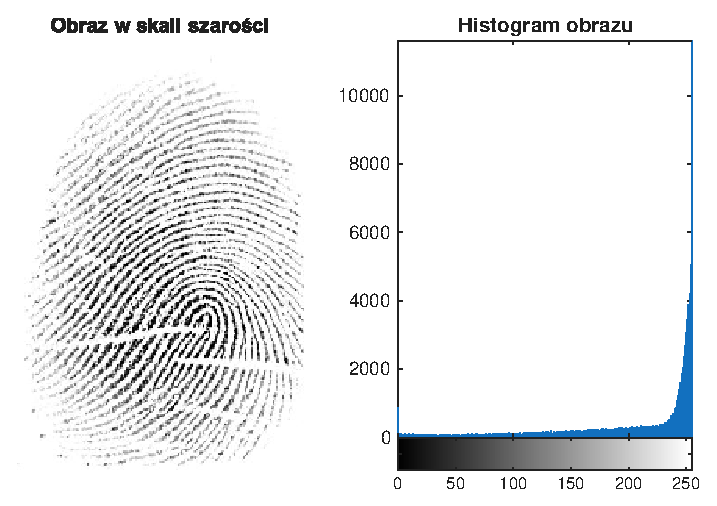
\includegraphics[width=0.7\linewidth]{figures/finger001.eps}\\
    \caption{Obraz wejściowy i jego histogram.\label{Wyniki001}}
\end{figure}

\subsection{Wyrównanie histogramu}
Przeprowadzono operację wyrównywania histogramu w celu poprawy kontrastu (patrz \listingname~\ref{Lab001_l2}):

\lstinputlisting[style= matlabStyle, caption= Wyrównanie histogramu, label=Lab001_l2]{src/Lab001/listing002.m}

\noindent Na \figurename~\ref{Wyniki002} przedstawiono otrzymane rezultaty po wyrównaniu histogramu.

\begin{figure}[H]
    \centering
    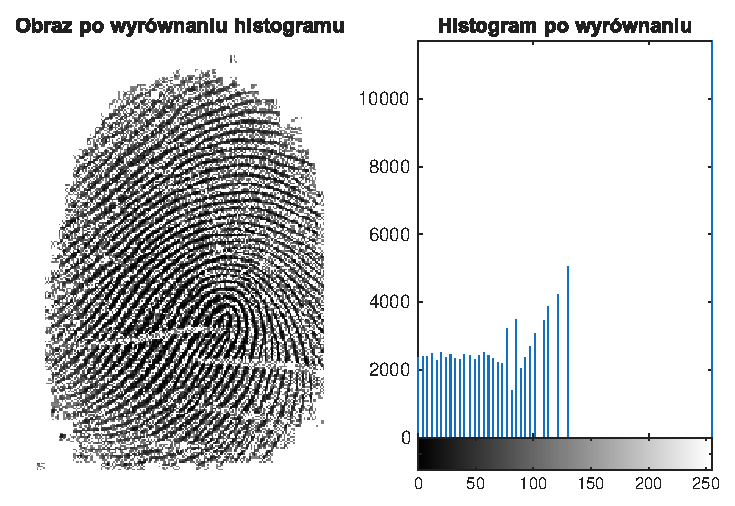
\includegraphics[width=0.7\linewidth]{figures/fingeHistogram.eps}\\
    \caption{Obraz po wyrównaniu i jego histogram.\label{Wyniki002}}
\end{figure}


\section{Wyniki i analiza}
Po przeprowadzeniu analizy histogramu uzyskano następujące wyniki:
\begin{itemize}
    \item Histogram oryginalnego obrazu wykazał skupienie wartości pikseli w wąskim zakresie, co wskazuje na niski kontrast.
    \item Po wyrównaniu histogramu kontrast obrazu uległ poprawie, a wartości pikseli zostały bardziej równomiernie rozłożone.
    \item Metoda Otsu pozwoliła na automatyczne wyznaczenie progu binaryzacji, co umożliwiło efektywne wydzielenie struktur biometrycznych na obrazie.
\end{itemize}

\section{Wnioski}
Na podstawie przeprowadzonych eksperymentów można stwierdzić, że:
\begin{itemize}
    \item Histogram jest przydatnym narzędziem w analizie jakości obrazu biometrycznego.
    \item Wyrównanie histogramu poprawia kontrast i może zwiększać czytelność obrazu.
    \item Segmentacja oparta na histogramie, w szczególności metoda Otsu, pozwala na skuteczne wydzielenie istotnych cech obrazu.
\end{itemize}

\section{Bibliografia}
\begin{itemize}
    \item MATLAB Image Processing Toolbox Documentation \cite{mathworks},
    \item Rafael Gonzalez, Richard Woods, Digital Image Processing Global Edition \cite{gonzalez2017}.
\end{itemize}
